%\newpage

\section{Problem Definition}
\label{sec:problem-definition}
%\guy{Can someone check Sections 3-4-5? Especially the formulations}

Our \toolname{} syntax is defined as follows: 
%of Fig.~\ref{fig:syntax}.

\[
\begin{aligned}
	\mathbf{Expression}\quad e ::={}&{} \\
	&0 \mid 1 \mid 2 \mid \dots 
	&&\grammartag{Numeric constants}\\
	&\nondet
	&&\grammartag{Nondeterministic value: 0 or 1}\\
	&x := e
	&&\grammartag{Write to local variable}\\
	&x
	&&\grammartag{Read from local variable}\\
	&X := e
	&&\grammartag{Write to global variable}\\
	&X
	&&\grammartag{Read from global variable}\\
	&e_1 == e_2
	&&\grammartag{Equality test}\\
	&e_1 ; e_2
	&&\grammartag{Sequencing}\\
	&\ifkw(e_1)\{e_2\}\elsekw\{e_3\}
	&&\grammartag{Conditional}\\
	&\whilekw(e_1)\{e_2\}
	&&\grammartag{While loop}\\
	&\yieldkw
	&&\grammartag{Yields to scheduler}\\[1em]
	\mathbf{Program}\quad p ::={}&{} \\
	&\requestkw\ name_1\{e_1\}
	&&\grammartag{Set of request handlers}\\
	&\quad\vdots\\
	&\requestkw\ name_n\{e_n\}
\end{aligned}
\]

%
%
%\begin{figure}[!htbp]
%    \begin{align*}
%    \mathbf{Expression}\quad e ::= &&& \\
%       | & \quad 0 \mid 1 \mid 2 \mid \ldots                                && \grammartag{Numeric constants} \\
%       | & \quad \nondet                                 && \grammartag{Nondeterministic value: 0 or 1}\\
%       | & \quad x := e                            && \grammartag{Write to local variable field} \\
%       | & \quad x                                 && \grammartag{Read from local variable field} \\
%       | & \quad X := e                            && \grammartag{Write to global  variable} \\
%       | & \quad X                                 && \grammartag{Read from global  variable} \\
%       | & \quad e_1 == e_2                        && \grammartag{Equality test} \\
%       | & \quad e_1 ; e_2                         && \grammartag{Sequencing} \\
%       | & \quad \ifkw(e_1)\{\ e_2\ \}\elsekw\{\ e_3\ \} && \grammartag{Conditional} \\
%       | & \quad \whilekw(e_1)\{\ e_2\ \}              && \grammartag{While loop} \\
%       | & \quad \yieldkw                      && \grammartag{Yields to scheduler}\\[1em]
%    \mathbf{Program}\quad p ::=
%        & \quad \requestkw\ name_1\ \{\ e_1\ \}&&\grammartag{Set of request handlers}\\[-0.5em]
%        & \quad \qquad \vdots &&\\
%        & \quad \requestkw\ name_n\ \{\ e_n\ \}\ 
%    \end{align*}
%    \caption{Syntax of expressians and programs}
%    \label{fig:syntax}
%\end{figure}
    %
This NS setting is motivated by software-defined networking. In the networking domain, spawning a request corresponds to sending a \textit{packet}, with each local variable mapped to a unique \textit{packet header field}; global variables correspond to variables on \textit{programmable switches}, as they are shared among all requests visiting the switch. Throughout this paper, we use the term \emph{request} to refer to a concurrent computation unit. 
    
   
A network system $\mathcal{N}$ is a tuple $(G, L, \mathit{REQ}, \mathit{RESP}, g_0, \delta, \mathit{req}, \mathit{resp})$ where:
\begin{itemize}
\item $G$ is a set of global states (assignments to all global variables)
\item $L$ is a set of local states (local variable values and remaining program to execute)
\item $\mathit{REQ}$ is a set of request types (each marked {\color{ForestGreen}$\blacklozenge_\text{req}$})
\item $\mathit{RESP}$ is a set of response types (each marked {\color{red}$\blacklozenge_\text{resp}$})
\item $g_0 \in G$ is the initial global state
\item $\mathit{req} \subseteq \mathit{REQ} \times L$ maps each request type to its initial local state
\item $\mathit{resp} \subseteq L \times \mathit{RESP}$ maps final local states to response types
\item $\delta \subseteq (G \times L) \times (G \times L)$ defines atomic execution steps that update both global and local state
\end{itemize}

\begin{definition}[Request and Response]
A \emph{request} ${\color{ForestGreen}\blacklozenge_\text{r}} \in \mathit{REQ}$ represents the initiation of a concurrent computation unit. Each request has an associated handler expression from the program syntax that defines its behavior.
A \emph{response} ${\color{red}\blacklozenge_\text{s}} \in \mathit{RESP}$ represents the value returned by a request after its execution terminates.
The pair $({\color{ForestGreen}\blacklozenge_\text{r}}, {\color{red}\blacklozenge_\text{s}}) \in \mathit{REQ} \times \mathit{RESP}$ captures the complete input-output behavior of a single request execution.
\end{definition}




\begin{figure}[t]
    \centering
    \renewcommand{\arraystretch}{1.6}
    \[
    \begin{array}{c}
    \textbf{States and Transitions:}
    \\
    \quad
    \text{A (global) \emph{network state} is a triple }(g,\mathcal{P},M)\text{ where:}
    \\
    \quad
    g \in G \text{ is the current global state,}
    \\
    \quad
    \mathcal{P} \in \text{Multiset}(L \times \mathit{REQ}) \text{ is a multiset of in-flight requests (threads),}
    \\
    \quad
    M \in \text{Multiset}(\mathit{REQ} \times \mathit{RESP}) \text{ is a multiset of request/response pairs already completed.}
    \end{array}
    \]

    \[
    \begin{array}{c}
    \textbf{Initial state:}
    \\
    \quad (g_0,\,\varnothing,\,\varnothing)
    \end{array}
    \]

    \[
    \begin{array}{c}
    \textbf{Transition rules:}
    \\[1em]
    \text{(New Request)}\quad\infer{
    ({\color{ForestGreen}\blacklozenge_\text{r}},\ell)\,\in\,\mathit{req}
    }
    {(g,\;\mathcal{P},\;M) \;\longrightarrow\; (g,\;\mathcal{P} \uplus \{(\ell,{\color{ForestGreen}\blacklozenge_\text{r}})\},\;M)}
    \\[2em]
    \text{(Processing Step)}\quad\infer{
    ((g,\ell),\,(g',\ell')) \,\in\, \delta
    }
    {(g,\;\mathcal{P} \uplus \{(\ell,{\color{ForestGreen}\blacklozenge_\text{r}})\},\;M) \;\longrightarrow\; (g',\;\mathcal{P} \uplus \{(\ell',{\color{ForestGreen}\blacklozenge_\text{r}})\},\;M)}
    \\[2em]
    \text{(Response)}\quad\infer{
    (\ell,{\color{red}\blacklozenge_\text{s}})\,\in\,\mathit{resp}
    }
    {(g,\;\mathcal{P} \uplus \{(\ell,{\color{ForestGreen}\blacklozenge_\text{r}})\},\;M) \;\longrightarrow\; (g,\;\mathcal{P},\;M \uplus \{({\color{ForestGreen}\blacklozenge_\text{r}},{\color{red}\blacklozenge_\text{s}})\})}
    \end{array}
    \]

    \[
    \begin{array}{c}
    \textbf{Complete runs:}
    \\
    \quad (g_0,\,\varnothing,\,\varnothing) \;\longrightarrow\; (g_1,\,\mathcal{P}_1,\,M_1) \;\longrightarrow\; \cdots \;\longrightarrow\; (g_n,\,\mathcal{P}_{n-1},\,M_{n-1}) \;\longrightarrow\; (g_n,\,\varnothing,\,M_n)
    \\[1em]
    \textbf{Interleaved run: } \text{the } \mathcal{P}_i \text{ can have more than one request, and } \mathcal{P}_n = \varnothing \\
    \textbf{Serial run: } \text{ each } \mathcal{P}_i \text{ has at most one request, and } \mathcal{P}_n = \varnothing\\
    \text{Int}(\mathcal{N}) = \{ M \in \text{Multiset}(\mathit{REQ} \times \mathit{RESP}) \mid \exists \text{ interleaved run } (g_0,\,\varnothing,\,\varnothing) \;\longrightarrow^*\; (g_n,\,\varnothing,\,M) \}\\
    \text{Ser}(\mathcal{N}) = \{ M \in \text{Multiset}(\mathit{REQ} \times \mathit{RESP}) \mid \exists \text{ serial run } (g_0,\,\varnothing,\,\varnothing) \;\longrightarrow^*\; (g_n,\,\varnothing,\,M) \}\\
    \end{array}
    \]

    \caption{State-transition rules for executions of
    \(\mathcal{N} = (G, L, \mathit{REQ}, \mathit{RESP}, g_0, \delta, \mathit{req}, \mathit{resp})\).
    A transition \(\longrightarrow\) modifies the triple \((g,\mathcal{P}, M)\) by either (1) introducing a new request, (2) processing a request step via \(\delta\), or (3) consuming a request to produce its response.  When no more steps are possible, the result set \(M\) is the final multiset of request/response pairs that arose during the run.
    Runs are called \emph{serial} if there is at most one request in flight at any time, whereas \emph{interleaved} runs may have multiple requests in flight at once.}
    \label{fig:network-transitions}
\end{figure}

\begin{definition}[Serializability]
A network system $\mathcal{N}$ is \emph{serializable} if $\text{Int}(\mathcal{N}) = \text{Ser}(\mathcal{N})$, meaning every multiset of request/response pairs attainable through an interleaved execution can also be achieved through some serial execution.
\end{definition}

\subsection{NS Example: Non-Serializability }
\label{sec:ns-non-serializable}

Recall the code snippet from the simple, non-serializable example presented in Listing~\ref{lst:MotivatingExample2NonSer}. We can represent its NS with the following mapping:

\begin{itemize}
\item 
The set $G$ is defined as $G=\{[\texttt{X=0}], [\texttt{X=1}]\}$

\item 
The initial global state is defined as $g_0 = [\texttt{X=0}]$.

\item 
We define $L$ as all pairs of local states (assignments such as $[\texttt{y=0}], [\texttt{y=1}]$) and ``remaining'' programs.

\item 
The set of requests is $REQ = \{{\color{ForestGreen}\blacklozenge_\text{main}}\}$

\item 
The set of responses is $RESP = \{{\color{red}\blacklozenge_0},{\color{red}\blacklozenge_1}\}$

\end{itemize}


We define the three mappings $req$, $resp$, and $\delta$ in Fig.~\ref{fig:code2ExampleNS}.
The figure also includes the explicit network system that
serves as a mapping from requests ({\color{ForestGreen}$\blacklozenge_\text{main}$}) to responses ({\color{red}$\blacklozenge_0$}, {\color{red}$\blacklozenge_1$}).
%
We note that we depicted only part of the states that are \textit{reachable}, in our finite-state setting.
%

\begin{figure}[!htbp]
	\centering
	%–––– Network system diagram ––––
	% \includegraphics[width=\textwidth]{plots/code_2_NS.png}\\[1ex]

	\begin{tikzpicture}[
		node distance=1.5cm and 2.5cm,
		>=stealth,
		thick,
		every node/.style={font=\small}
	]
	  % [main request] -> [y=0][full program below that] ---[X=1 -> X=1][X=0 -> X=1 below that]--->[y=0][rest of program below that]
	  %   (first outgoing edge of last node on previous line)
      %   --[X=0 -> X=0]-->[y=0][empty program below that] ---> [0 response]
	  %   (second outgoing edge)
	  %   --[X=1 -> X=0]-->[y=1][empty program below that] ---> [1 response]
	  
	  % Main request node
	  \node[
		draw=black,
		line width=0.8pt,
		fill=ForestGreen!20,
		text=black,
		diamond,
		aspect=2,
		inner sep=2pt,
		scale=0.7
	  ] (main) {\texttt{main}};
	  
	  % First state node with full program
	  \node[right=0.7cm of main, align=center] (state1) {
		\begin{tikzpicture}[baseline=(ybox.base)]
			\node[
			draw=black,
			line width=0.8pt,
			fill=brightyellow,
			text=black,
			rectangle,
			rounded corners=1pt,
			inner sep=2pt
			] (ybox) {\texttt{y=0}};
		\end{tikzpicture}\\[-2.5pt]
		\begin{minipage}{2cm}
			\begin{lstlisting}[language=CustomPseudoCode,numbers=none,basicstyle=\tiny\ttfamily]
X := 1
yield
y := X + 1
X := 0
return y
			\end{lstlisting}
		\end{minipage}
	  };
	  
	  % Second state node with rest of program
	  \node[right=of state1, align=center] (state2) {
		\begin{tikzpicture}[baseline=(ybox.base)]
			\node[
			draw=black,
			line width=0.8pt,
			fill=brightyellow,
			text=black,
			rectangle,
			rounded corners=1pt,
			inner sep=2pt
			] (ybox) {\texttt{y=0}};
		\end{tikzpicture}\\[-2.5pt]
		\begin{minipage}{1.5cm}
			\begin{lstlisting}[language=CustomPseudoCode,numbers=none,basicstyle=\tiny\ttfamily]
y := X + 1
X := 0
return y
			\end{lstlisting}
		\end{minipage}
	  };
	  
	  % Final state y=0 with empty program
	  \node[above right=-0.5cm and 2.2cm of state2, align=center] (state3) {
		\begin{tikzpicture}[baseline=(ybox.base)]
			\node[
			draw=black,
			line width=0.8pt,
			fill=brightyellow,
			text=black,
			rectangle,
			rounded corners=1pt,
			inner sep=2pt
			] (ybox) {\texttt{y=0}};
		\end{tikzpicture}\\[-2.5pt]
		\begin{minipage}{0.8cm}
			\begin{lstlisting}[language=CustomPseudoCode,numbers=none,basicstyle=\tiny\ttfamily]
// end
			\end{lstlisting}
		\end{minipage}
	  };
	  
	  % Final state y=1 with empty program
	  \node[below right=-0.2cm and 2.2cm of state2, align=center] (state4) {
		\begin{tikzpicture}[baseline=(ybox.base)]
			\node[
			draw=black,
			line width=0.8pt,
			fill=brightyellow,
			text=black,
			rectangle,
			rounded corners=1pt,
			inner sep=2pt
			] (ybox) {\texttt{y=1}};
		\end{tikzpicture}\\[-2.5pt]
		\begin{minipage}{0.8cm}
			\begin{lstlisting}[language=CustomPseudoCode,numbers=none,basicstyle=\tiny\ttfamily]
// end
			\end{lstlisting}
		\end{minipage}
	  };
	  
	  % Response 0
	  \node[
		right=0.6cm of state3,
		draw=black,
		line width=0.8pt,
		fill=RedViolet!20,
		text=black,
		diamond,
		aspect=2,
		inner sep=2pt,
		scale=0.7,
		font=\Large
	  ] (resp0) {\texttt{0}};
	  
	  % Response 1
	  \node[
		right=0.6cm of state4,
		draw=black,
		line width=0.8pt,
		fill=RedViolet!20,
		text=black,
		diamond,
		aspect=2,
		inner sep=2pt,
		scale=0.7,
		font=\Large
	  ] (resp1) {\texttt{1}};
	  
	  % Arrows
	  \draw[->] (main) -- (state1);
	  
	  % Transition labels for state1 to state2
	  \draw[->] (state1) -- node[above] {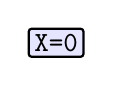
\begin{tikzpicture}[baseline=(a.base)]\node[draw=black,line width=0.8pt,fill=blue!10,rectangle,rounded corners=1pt,inner sep=2pt] (a) {\texttt{X=0}};\end{tikzpicture} $\to$ 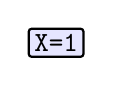
\begin{tikzpicture}[baseline=(b.base)]\node[draw=black,line width=0.8pt,fill=blue!10,rectangle,rounded corners=1pt,inner sep=2pt] (b) {\texttt{X=1}};\end{tikzpicture}} node[below] {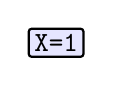
\begin{tikzpicture}[baseline=(c.base)]\node[draw=black,line width=0.8pt,fill=blue!10,rectangle,rounded corners=1pt,inner sep=2pt] (c) {\texttt{X=1}};\end{tikzpicture} $\to$ 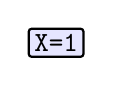
\begin{tikzpicture}[baseline=(d.base)]\node[draw=black,line width=0.8pt,fill=blue!10,rectangle,rounded corners=1pt,inner sep=2pt] (d) {\texttt{X=1}};\end{tikzpicture}} (state2);
	  
	  % From state2 to final states
	  \draw[->] ([yshift=4pt]state2.east) to[out=50,in=180] node[above, sloped] {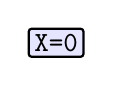
\begin{tikzpicture}[baseline=(a.base)]\node[draw=black,line width=0.8pt,fill=blue!10,rectangle,rounded corners=1pt,inner sep=2pt] (a) {\texttt{X=0}};\end{tikzpicture} $\to$ 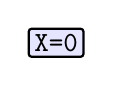
\begin{tikzpicture}[baseline=(b.base)]\node[draw=black,line width=0.8pt,fill=blue!10,rectangle,rounded corners=1pt,inner sep=2pt] (b) {\texttt{X=0}};\end{tikzpicture}} (state3.west);
	  \draw[->] ([yshift=-16pt]state2.east) to[out=-50,in=180] node[below, sloped] {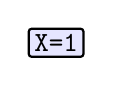
\begin{tikzpicture}[baseline=(a.base)]\node[draw=black,line width=0.8pt,fill=blue!10,rectangle,rounded corners=1pt,inner sep=2pt] (a) {\texttt{X=1}};\end{tikzpicture} $\to$ 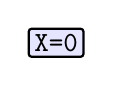
\begin{tikzpicture}[baseline=(b.base)]\node[draw=black,line width=0.8pt,fill=blue!10,rectangle,rounded corners=1pt,inner sep=2pt] (b) {\texttt{X=0}};\end{tikzpicture}} (state4.west);
	  
	  % To responses
	  \draw[->] (state3) -- (resp0);
	  \draw[->] (state4) -- (resp1);
	  
	\end{tikzpicture}
	
	%–––– req, resp, and δ definitions ––––
	\[
	\begin{array}{@{}r@{\;}l}
	req \coloneq & 
	\big\{
	\big[
	\begin{array}{c c c}
		\begin{tikzpicture}[baseline=(textnode.base)]
			\node[
			draw=black,
			line width=0.8pt,
			fill=ForestGreen!20,
			text=black,
			diamond,
			aspect=2,
			inner sep=2pt,
			scale=0.7
			] (textnode) {\texttt{main}};
		\end{tikzpicture}
		&\!\!\rightarrow\!\!&
		\begin{array}{c}
			\begin{tikzpicture}[baseline=(ybox.base)]
				\node[
				draw=black,
				line width=0.8pt,
				fill=brightyellow,
				text=black,
				rectangle,
				rounded corners=1pt,
				inner sep=2pt
				] (ybox) {\texttt{y=0}};
			\end{tikzpicture}\vspace{-2pt}
			\\
			\begin{minipage}{0.20\linewidth}
				\begin{lstlisting}[language=CustomPseudoCode,numbers=none,basicstyle=\tiny\ttfamily]
X := 1 
yield 
y := X + 1
X := 0
return y
				\end{lstlisting}
			\end{minipage}
		\end{array}
	\end{array}
	\big]
	\big\}
	\\[2em]
	resp \coloneq &
	\big\{
	\big[
	\begin{array}{c c c}
		\begin{array}{c}
			\begin{tikzpicture}[baseline=(ybox.base)]
				\node[
				draw=black,
				line width=0.8pt,
				fill=brightyellow,
				text=black,
				rectangle,
				rounded corners=1pt,
				inner sep=2pt
				] (ybox) {\texttt{y=0}};
			\end{tikzpicture}\vspace{-2pt}
			\\
			\begin{minipage}{0.11\linewidth}
				\begin{lstlisting}[language=CustomPseudoCode,numbers=none,basicstyle=\tiny\ttfamily]
// end
				\end{lstlisting}
			\end{minipage}
		\end{array}
		&\!\!\rightarrow\!\!&
		\begin{tikzpicture}[baseline=(textnode.base),scale=0.7]
			\node[
			draw=black,
			line width=0.8pt,
			fill=RedViolet!20,
			text=black,
			diamond,
			aspect=2,
			inner sep=2pt,
			font=\small
			] (textnode) {\texttt{0}};
		\end{tikzpicture}
	\end{array}
	\big]\,{},
	\big[
	\begin{array}{c c c}
		\begin{array}{c}
			\begin{tikzpicture}[baseline=(ybox.base)]
				\node[
				draw=black,
				line width=0.8pt,
				fill=brightyellow,
				text=black,
				rectangle,
				rounded corners=1pt,
				inner sep=2pt
				] (ybox) {\texttt{y=1}};
			\end{tikzpicture}\vspace{-2pt}
			\\
			\begin{minipage}{0.11\linewidth}
				\begin{lstlisting}[language=CustomPseudoCode,numbers=none,basicstyle=\tiny\ttfamily]
// end
				\end{lstlisting}
			\end{minipage}
		\end{array}
		&\!\!\rightarrow\!\!&
		\begin{tikzpicture}[baseline=(textnode.base),scale=0.7]
			\node[
			draw=black,
			line width=0.8pt,
			fill=RedViolet!20,
			text=black,
			diamond,
			aspect=2,
			inner sep=2pt,
			font=\small
			] (textnode) {\texttt{1}};
		\end{tikzpicture}
	\end{array}
	\big]
	\big\}
	\\[2em]
	\delta \coloneq & 
	\big\{\big[(
		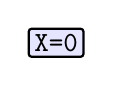
\begin{tikzpicture}[baseline=(ybox.base)]
			\node[
			draw=black,
			line width=0.8pt,
			fill=blue!10,
			text=black,
			rectangle,
			rounded corners=1pt,
			inner sep=2pt
			] (ybox) {\texttt{X=0}};
		\end{tikzpicture}\,{},
		\begin{array}{c}
			\begin{tikzpicture}[baseline=(ybox.base)]
				\node[
				draw=black,
				line width=0.8pt,
				fill=brightyellow,
				text=black,
				rectangle,
				rounded corners=1pt,
				inner sep=2pt
				] (ybox) {\texttt{y=0}};
			\end{tikzpicture}\vspace{-2pt}
			\\
			\begin{minipage}{0.14\linewidth}
				\begin{lstlisting}[language=CustomPseudoCode,numbers=none,basicstyle=\tiny\ttfamily]
X := 1
yield
y := X + 1
X := 0
return y
				\end{lstlisting}
			\end{minipage}
		\end{array}
		)
		\;\rightarrow\;
		(
		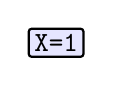
\begin{tikzpicture}[baseline=(ybox.base)]
			\node[
			draw=black,
			line width=0.8pt,
			fill=blue!10,
			text=black,
			rectangle,
			rounded corners=1pt,
			inner sep=2pt
			] (ybox) {\texttt{X=1}};
		\end{tikzpicture}\,{},
		\begin{array}{c}
			\begin{tikzpicture}[baseline=(ybox.base)]
				\node[
				draw=black,
				line width=0.8pt,
				fill=brightyellow,
				text=black,
				rectangle,
				rounded corners=1pt,
				inner sep=2pt
				] (ybox) {\texttt{y=0}};
			\end{tikzpicture}\vspace{-2pt}
			\\
			\begin{minipage}{0.14\linewidth}
				\begin{lstlisting}[language=CustomPseudoCode,numbers=none,basicstyle=\tiny\ttfamily]
y := X + 1
X := 0
return y
				\end{lstlisting}
			\end{minipage}
		\end{array}
		)
		\big],
	\\[0.5em]
	& \phantom{\big\{}
		\big[(
		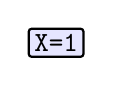
\begin{tikzpicture}[baseline=(ybox.base)]
			\node[
			draw=black,
			line width=0.8pt,
			fill=blue!10,
			text=black,
			rectangle,
			rounded corners=1pt,
			inner sep=2pt
			] (ybox) {\texttt{X=1}};
		\end{tikzpicture}\,{},
		\begin{array}{c}
			\begin{tikzpicture}[baseline=(ybox.base)]
				\node[
				draw=black,
				line width=0.8pt,
				fill=brightyellow,
				text=black,
				rectangle,
				rounded corners=1pt,
				inner sep=2pt
				] (ybox) {\texttt{y=0}};
			\end{tikzpicture}\vspace{-2pt}
			\\
			\begin{minipage}{0.14\linewidth}
				\begin{lstlisting}[language=CustomPseudoCode,numbers=none,basicstyle=\tiny\ttfamily]
y := X + 1
X := 0
return y
				\end{lstlisting}
			\end{minipage}
		\end{array}
		)
		\;\rightarrow\;
		(
		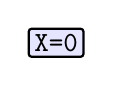
\begin{tikzpicture}[baseline=(ybox.base)]
			\node[
			draw=black,
			line width=0.8pt,
			fill=blue!10,
			text=black,
			rectangle,
			rounded corners=1pt,
			inner sep=2pt
			] (ybox) {\texttt{X=0}};
		\end{tikzpicture}\,{},
		\begin{array}{c}
			\begin{tikzpicture}[baseline=(ybox.base)]
				\node[
				draw=black,
				line width=0.8pt,
				fill=brightyellow,
				text=black,
				rectangle,
				rounded corners=1pt,
				inner sep=2pt
				] (ybox) {\texttt{y=1}};
			\end{tikzpicture}
			\vspace{-2pt}
			\\
			\begin{minipage}{0.11\linewidth}
				\begin{lstlisting}[language=CustomPseudoCode,numbers=none,basicstyle=\tiny\ttfamily]
// end
				\end{lstlisting}
			\end{minipage}
		\end{array}
		)
		\big],
		\ldots
	\big\}
	\end{array}
	\]
	\caption{Network system and transition functions for the program in Listing~\ref{lst:MotivatingExample2NonSer}.}
\label{fig:code2ExampleNS}
\end{figure}


